% !TEX program = xelatex
\documentclass{article}
\usepackage{geometry}
\geometry{left = 3cm, right = 3cm, top = 3cm, bottom = 3cm}
\usepackage[linesnumbered,ruled,longend]{algorithm2e}
\usepackage{amsmath}
\usepackage{amsfonts,amssymb}
\usepackage{blkarray}
\usepackage{booktabs}
\usepackage{dsfont}
\usepackage{enumerate}
\usepackage{epsf}
\usepackage{fontspec}
\usepackage{forest}
\usepackage[colorlinks=true,linkcolor=purple]{hyperref}
\usepackage{listings}
\usepackage{mathrsfs}
\usepackage{microtype}
\usepackage{multirow}
\usepackage{setspace}
\usepackage{tikz}
%\usepackage{indentfirst}
%\usepackage[usenames,dvipsnames]{xcolor}
\newfontfamily\Inputmono{Consolas}
\renewcommand\thesection{Question\ \arabic{section}}%\arabic{section}}
\renewcommand\thesubsection{(\arabic{subsection})}
\renewcommand\thesubsubsection{\arabic{subsubsection}.}
\newcommand{\qedhere}{$\hfill\ensuremath{\square}$}
\defaultfontfeatures{Mapping=tex-text,Scale=MatchLowercase}
\newcommand\mycommfont[1]{\ttfamily\textcolor{blue}{#1}}
\SetCommentSty{mycommfont}
%\setmainfont{Citadel Script}
%\setmainfont{Chalkboard}
\setmainfont{CMU Bright}
%\setmainfont{Apple Chancery}
\setmonofont{Optima}
\setsansfont{Optima}
%\renewcommand{\familydefault}{\sfdefault}
%\renewcommand{\footnotesize}{\sfdefault}
\setlength{\parskip}{0.25em}
\setlength{\parindent}{0em}

%%%%%%%%%%%Configurations for code%%%%%%%%%%%%%%%%%%%%%%%
\SetKwInOut{Input}{Input}
\SetKwInOut{Output}{Output}
\SetKwProg{Fn}{Function}{\string:}{end}
\SetKwFunction{mstnew}{MST\_New}
\SetKwFunction{tw}{TreeWeight}
\SetKwFunction{dps}{DFS}
\SetKwFunction{con}{Is\_Connected}
\SetKwFunction{hor}{Three\_Fastest\_Horses}
%%%%%%%%%%%Here is the configurations for Code%%%%%%%%%%%

%\definecolor{mygreen}{rgb}{0,0.6,0}
%\definecolor{mygray}{rgb}{0.7,0.7,0.7}
%\definecolor{mymauve}{rgb}{0.58,0,0.82}
%\definecolor{mywhite}{rgb}{1,1,1}
%\definecolor{myblack}{rgb}{0,0,0}
%\definecolor{myblue}{RGB}{27,154,154}
%\lstset{
% backgroundcolor=\color{white},
% basicstyle = \footnotesize\Inputmono,
% breakatwhitespace = false,
% breaklines = true,
% captionpos = b,
% commentstyle = \color{mygray}\bfseries,
% extendedchars = false,
% frame =shadowbox,
% framerule=0.5pt,
% frameround=tttt,
% keepspaces=true,
% keywordstyle=\color{myblue}\bfseries, % keyword style
% language = Verilog,                     % the language of code
% otherkeywords={string},
% numbers=left,
% numbersep=5pt,
% numberstyle=\tiny\color{mymauve},
% rulecolor=\color{black},
% showspaces=false,
% showstringspaces=false,
% showtabs=false,
% stepnumber=0,
% stringstyle=\color{mymauve},        % string literal style
% tabsize=2,
% title=\lstname
%}

%%%%%%%%%%%%%%%%%%%%%%%%%%%%%%%%%%%%%%%%%%%%

\begin{document}
%\setmainfont{Savoye LET}
%\setmainfont{Cormorant Upright}
\setmainfont{Cormorant Upright}
\renewcommand\arraystretch{1.5}


\thispagestyle{empty}

\begin{center}
\begin{large}
\begin{figure}[!htbp]
\centering

\includegraphics[width=0.7\textwidth]{Logo2}
\end{figure}
\hrule
\vspace*{0.25cm}
\sc{ \Large  UM--SJTU Joint Institute \vspace*{0.3em}} \\
\Large  VE477 Intro to Algorithms\\
\end{large}
\hrulefill

\vspace*{3cm}

\begin{Large}
\sc{{Homework 8}} \\
\end{Large}
\vspace*{2cm}
\begin{large}
\sc{{Wang, Tianze\\ 515370910202}} \\
\end{large}
\end{center}
\newpage
\setmainfont{Optima}
\setmonofont{Optima}
\setsansfont{Optima}
%\tableofcontents
%\newpage
\setcounter{page}{1}
\section{Fast multi-point evaluation and interpolation - Part I}
\subsection{Binary tree}
\begin{center}
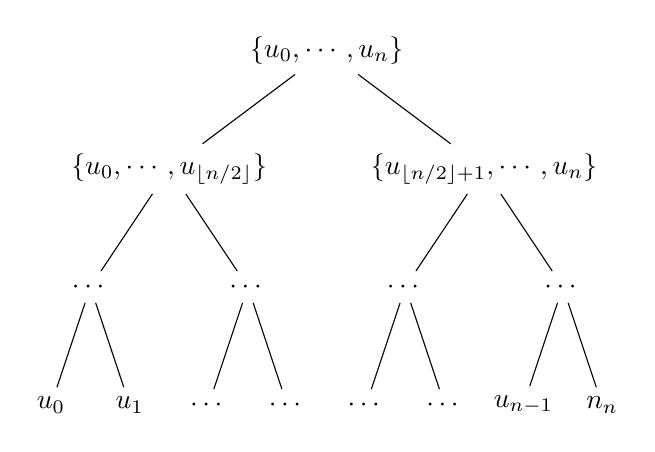
\begin{tikzpicture} 
\tikzstyle{level 1}=[sibling distance=40mm]
\tikzstyle{level 2}=[sibling distance=20mm]
\tikzstyle{level 3}=[sibling distance=10mm]
\node {$\{u_0, \cdots, u_n\}$}
child {node {$\{u_0, \cdots, u_{\lfloor n/2 \rfloor }\}$}
	child {node { $\cdots$}
		child {node {$u_0$}}
		child {node {$u_1$}}
	}
	child {node { $\cdots$}
		child {node { $\cdots$}}
		child {node { $\cdots$}}
	}
}
child {node {$\{ u_{\lfloor n/2 \rfloor+1}, \cdots,u_n\}$}
	child {node { $\cdots$}
		child {node { $\cdots$}}
		child {node { $\cdots$}}
	}
	child {node { $\cdots$}
		child {node { $u_{n-1}$}}
		child {node { $n_{n}$}}
	}
};
\end{tikzpicture}
\end{center}
\subsection{Prove $M_{i,j}$}
The base case is easy to prove:
\begin{align*}
M_{0,j} &= \prod_{l=0}^{2^1-1} m_{j\cdot 2^0 + l} \\
		&= \prod_{l=0}^{0} m_{j\cdot 2^0 + l} \\
		&= m_{j+0} \\
		&= m_j
\end{align*}

For $0 \leq i < k$,
\begin{align*}
	M_{i+1,j} &= \prod_{l=0}^{2\cdot 2^i-1} m_{j\cdot 2^i+l}\\
			  &= \prod_{l=0}^{ 2^i-1} m_{j\cdot 2^i+l}\cdot \prod_{l=2^i}^{2\cdot 2^i-1} m_{j\cdot 2^i+l}\\
			  &= \prod_{l=0}^{ 2^i-1} m_{j\cdot 2^i+l}\cdot \prod_{l=0}^{ 2^i-1} m_{j\cdot 2^i+2^i+l}\\
			  &= M_{i,2j} \cdot M_{i, 2j+1}
\end{align*}
\qedhere
\subsection{$M_{i,j}$ and binary tree}
$M_{i,j}$ means that, if the $j^{th}$ set in $i^{th}$ level has an element evaluated as 0, then $M_{i,j} = 0$.
\newpage
\subsection{Fast Multipoint Evaluation}
\subsubsection*{Algorithm build subtree and return polynomials}
\begin{algorithm}
\Input{$U = {u_0,u_1,...,u_n}$}
\Output{Subproduct tree}
\SetKwFunction{fd}{Algo1}
\Fn{\fd{$U$}}{
	$k \leftarrow log_2 n +1$\;
	\For{i in (0, k+1)}{
		\For{j in (0, $2^{k-i}$)}{
			\uIf{i = 0}{
				\KwRet{$M_{i,j} = X - u_{i,j}$}
			}
			\Else{
				\KwRet{$M_{i,j} = M_{i-1, 2j} M_{i-1, 2j+1}$}
			}
		}
	}
}
\end{algorithm}

\subsubsection*{Recursive algo}

\subsection{Correctness}
\begin{enumerate}[a.]
\item Base case: $k=0$, the polynomial is a constant, and the algorithm will correctly return this value, so it is true. Suppose it holds for $k = a$, then for $k = a+1$, since the return value are true for all the results from $k=a$, and $k=a+1$ is the combination (Union operation) of the result from $k=a$, which means it also returns the correct value. proved
\item Since the operation is 
\[
	T(2^k) = 2\cdot T(2^{k-1}) + f(2^{k-1})
\]
According to Master Theorem, $T(n) = \mathcal{O}(M(n) \cdot \log n)$
\end{enumerate}

\section*{Part II}

\Huge \textbf{Well, fuck it off!}
\normalsize
\section{Critical Thinking}
\subsection{Abelian group}
\subsection{Two sb students}
First list all the primes smaller than 100:
2, 3, 5, 7, 11, 13, 17, 19, 23, 29, 31, 37, 41, 43, 47, 53, 59, 61, 67, 71, 73, 79, 83, 89, 97
\begin{enumerate}
\item The first sentence by the first student indicates that these cannot be product of two primes. So the number known by the first student cannot be from: 4, 6, 9, 10, 14, 15, 21, 22, 25, 26, 33, 34, 35, 38, 39, 46, 49, 51, 55, 57, 58, 62, 65, 69, 74, 77, 82, 85, 86, 87, 91, 93, 94, 95
\item Then S2 says, `I know you couldn't know'. This is the trickiest part, which means the sum of the number cannot be the sum of two primes, otherwise chances are that S1 could know. Then we can see S1 only knows one from:
11, 17, 23, 27, 29, 35, 37, 41, 47, 51, 53, 57, 59, 65, 67, 71, 77, 79, 83, 87, 89, 93, 95, 97
\item After knowing this information, S1 knows the answer. Then we start by testing from 11.
\item $11=2+9=3+8=5+6$, all three combinations are fine, for $5+6$, after knowing the list from 11 to 97, the student could tell. We still need check $2+9$ and $3+8$. For $2+9$, the $3+6 = 9$ will lead to ambiguition, that's not excludable. So this is discarded.
\item $17 = 2+15 = 12 + 5 = 14 + 3$, After double check, we will find that only $14+3$ will be a possible combination, which means the two scores are $3$ and $14$.
\end{enumerate}
\subsection{Ant movement}
It makes no change whether there is a collide or not, since their speed are the same and the total system is not different from what it originally is than after the collision. So the time will then be the longest time for all the ants to get down from the string, which means
\[
	t_{max} = \frac{1}{1} = 1 (seconds)
\]	
\end{document}



